% This is "sig-alternate.tex" V2.1 April 2013
% This file should be compiled with V2.5 of "sig-alternate.cls" May 2012
%
% This example file demonstrates the use of the 'sig-alternate.cls'
% V2.5 LaTeX2e document class file. It is for those submitting
% articles to ACM Conference Proceedings WHO DO NOT WISH TO
% STRICTLY ADHERE TO THE SIGS (PUBS-BOARD-ENDORSED) STYLE.
% The 'sig-alternate.cls' file will produce a similar-looking,
% albeit, 'tighter' paper resulting in, invariably, fewer pages.
%
% ----------------------------------------------------------------------------------------------------------------
% This .tex file (and associated .cls V2.5) produces:
%       1) The Permission Statement
%       2) The Conference (location) Info information
%       3) The Copyright Line with ACM data
%       4) NO page numbers
%
% as against the acm_proc_article-sp.cls file which
% DOES NOT produce 1) thru' 3) above.
%
% Using 'sig-alternate.cls' you have control, however, from within
% the source .tex file, over both the CopyrightYear
% (defaulted to 200X) and the ACM Copyright Data
% (defaulted to X-XXXXX-XX-X/XX/XX).
% e.g.
% \CopyrightYear{2007} will cause 2007 to appear in the copyright line.
% \crdata{0-12345-67-8/90/12} will cause 0-12345-67-8/90/12 to appear in the copyright line.
%
% ---------------------------------------------------------------------------------------------------------------
% This .tex source is an example which *does* use
% the .bib file (from which the .bbl file % is produced).
% REMEMBER HOWEVER: After having produced the .bbl file,
% and prior to final submission, you *NEED* to 'insert'
% your .bbl file into your source .tex file so as to provide
% ONE 'self-contained' source file.
%
% ================= IF YOU HAVE QUESTIONS =======================
% Questions regarding the SIGS styles, SIGS policies and
% procedures, Conferences etc. should be sent to
% Adrienne Griscti (griscti@acm.org)
%
% Technical questions _only_ to
% Gerald Murray (murray@hq.acm.org)
% ===============================================================
%
% For tracking purposes - this is V2.0 - May 2012

\documentclass{elsarticle}




%\usepackage{color}
\usepackage{url}
\usepackage[usenames,dvipsnames,svgnames,table]{xcolor}
\usepackage{listings}
\usepackage{hyperref}
\usepackage{longtable} % or pandoc
\usepackage{booktabs}
\definecolor{StringRed}{rgb}{.637,0.082,0.082}
\definecolor{CommentGreen}{rgb}{0,0.5,0}
\definecolor{KeywordBlue}{rgb}{0,0,1}
\definecolor{UserTypeTeal}{rgb}{0.1679,0.5664,0.6836}

\lstdefinelanguage{threeextensions}%
  {morekeywords={var,from,select,where,orderby,yield,let,join,on,into,Equal,group,by,ascending,descending,
                 try,catch,finally},
   sensitive,
  }[keywords]%

\lstdefinelanguage{fourextensions}
   {morekeywords={dynamic},
    sensitive
   }[keywords]

\lstdefinelanguage{fiveextensions}
   {morekeywords={await,async},
    sensitive
   }[keywords]

\lstdefinelanguage{CSharpLatest}
                         {language=[Sharp]{C}, %
                          alsolanguage=threeextensions,
                          alsolanguage=fourextensions,
					alsolanguage=fiveextensions,
                          basicstyle=\color{black}\ttfamily\small,
                          showstringspaces=false,
                          keywordstyle=\color{KeywordBlue},
                          commentstyle=\color{CommentGreen},
                          stringstyle=\color{StringRed},
rangebeginprefix=\#region\ ,
rangeendprefix=\#endregion\ ,
includerangemarker=false,
                          columns=flexible
                         }

\lstdefinelanguage{conceptextensions}
   {morekeywords={instance,concept,interface,member,Witness,Trait,abstract,struct},
    sensitive
   }[keywords]
\lstdefinelanguage{FSharp}
                         {language={Caml}, %
                          alsolanguage=conceptextensions,
                          basicstyle=\color{black}\ttfamily\small,
                          showstringspaces=false,
                          keywordstyle=\color{KeywordBlue},
                          commentstyle=\color{CommentGreen},
                          stringstyle=\color{StringRed},
                          columns=flexible
                         }


\lstset{moredelim=[is][\color{UserTypeTeal}]{|}{|}}

\newif\ifclassic
\classicfalse

\begin{document}

%\setcopyright{none}
% Copyright
%\setcopyright{acmcopyright}
%\setcopyright{acmlicensed}
%\setcopyright{rightsretained}
%\setcopyright{usgov}
%\setcopyright{usgovmixed}
%\setcopyright{cagov}
%\setcopyright{cagovmixed}

%
% --- Author Metadata here ---
%\conferenceinfo{ML Workshop 2016}{Japan}
%\CopyrightYear{2007} % Allows default copyright year (20XX) to be over-ridden - IF NEED BE.
%\crdata{0-12345-67-8/90/01}  % Allows default copyright data (0-89791-88-6/97/05) to be over-ridden - IF NEED BE.
% --- End of Author Metadata ---

\begin{frontmatter}
\title{Classes for the Masses (Extended Abstract)  }   
\author{Claudio V. Russo}
\address{Microsoft Research Ltd, Cambridge, U.K.}
\author{Matthew Windsor}
\address{University of York}
 
%\titlenote{A full version of this paper is available as
%\textit{Author's Guide to Preparing ACM SIG Proceedings Using
%\LaTeX$2_\epsilon$\ and BibTeX} at
%\texttt{www.acm.org/eaddress.htm}}}
%
% You need the command \numberofauthors to handle the 'placement
% and alignment' of the authors beneath the title.
%
% For aesthetic reasons, we recommend 'three authors at a time'
% i.e. three 'name/affiliation blocks' be placed beneath the title.
%
% NOTE: You are NOT restricted in how many 'rows' of
% "name/affiliations" may appear. We just ask that you restrict
% the number of 'columns' to three.
%
% Because of the available 'opening page real-estate'
% we ask you to refrain from putting more than six authors
% (two rows with three columns) beneath the article title.
% More than six makes the first-page appear very cluttered indeed.
%
% Use the \alignauthor commands to handle the names
% and affiliations for an 'aesthetic maximum' of six authors.
% Add names, affiliations, addresses for
% the seventh etc. author(s) as the argument for the
% \additionalauthors command.
% These 'additional authors' will be output/set for you
% without further effort on your part as the last section in
% the body of your article BEFORE References or any Appendices.

%\numberofauthors{5} %  in this sample file, there are a *total*
% of EIGHT authors. SIX appear on the 'first-page' (for formatting
% reasons) and the remaining two appear in the \additionalauthors section.
%
%\author{
% You can go ahead and credit any number of authors here,
% e.g. one 'row of three' or two rows (consisting of one row of three
% and a second row of one, two or three).
%
% The command \alignauthor (no curly braces needed) should
% precede each author name, affiliation/snail-mail address and
% e-mail address. Additionally, tag each line of
% affiliation/address with \affaddr, and tag the
% e-mail address with \email.
%
% 1st. author
%\alignauthor
%Claudio Russo\\ \affaddr{(Microsoft Research)}
%% 2nd. author
%\alignauthor
%Matt Windsor\\ \affaddr{(University of York)}
%\and
%\alignauthor
%Don Syme\\  \affaddr{(Microsoft Research)}
%\alignauthor
%Rupert Horlick\\   \affaddr{(University of Cambridge)}
%\alignauthor
%James Clarke\\ \affaddr{(University of Cambridge)}
%}
%\alignauthor
%Claudio Russo\\
%% 2nd. author
%\alignauthor
%Matt Windsor\\
%\alignauthor
%Don Syme\\
%\alignauthor
%Rupert Horlick\\
%\alignauthor
%James Clarke\\
%% 2nd. author
%\and
%\alignauthor
% \affaddr{(Microsoft Research)}\\
%\alignauthor
%  \affaddr{(University of Cambridge)}\\
%\alignauthor
% \affaddr{(University of Cambridge)}\\
%}



\begin{abstract}
Type classes are an immensely popular and productive feature of Haskell. They have since been adopted in, and adapted to, numerous other languages, including theorem provers.
We show that type classes have a natural and efficient representation in .NET that paves the way for the extension of F\#, C\# and other .NET languages with type classes. 
Our encoding  is type preserving and promises easy and safe cross-language inter-operation.
We have extended the open source C\# compiler and language service, Roslyn, with pervasive support for type classes and  have prototyped a more minimalist design  for F\#.
\end{abstract}
\end{frontmatter}

% We no longer use \terms command
%\terms{Theory}

%\renewcommand{\subsection}{1}{}

\section{Introduction}

Haskell's \emph{type classes} \cite{peytonjones:h98,WadlerBlott} are a powerful abstraction mechanism for describing generic algorithms applicable to types that have different representations but common interfaces.
A \emph{type class} is a predicate on types that specifies a set of required operations by their type signatures with  optional, default code.
A type may be declared to be an \emph{instance} of a type class, and must supply an implementation for each of the class' operations. 
Type classes may be arranged hierarchically, permitting subsumption and inheritance. 
%A default implementation may also be associated with an operation. % allowing its implementations to be omitted.

Many modern languages have adopted features inspired
by type classes, with different implementation techniques.  Scala has
\emph{implicits}\cite{scalaimplicits}, implicit method arguments denoting dictionaries, that
are inferred by the compiler but represented, at run-time, as additional
heap-allocated arguments to methods (with commensurate overhead).  C++ came very
close to adopting \emph{concepts}\cite{cppconcepts}, a rather different extension of the template mechanism, 
directly inspired by Haskell's type classes but enforcing  compile-time code specialization for performance. Rust has \emph{traits}\cite{Rust}. Swift has
\emph{protocols}\cite{Swift}.

{\bf Contribution} We describe a simple encoding that allows us to add type classes to
any .NET language, allowing interoperable definitions of type
classes. Our encoding relies on the CLR's distinctive approach to
representing and compiling generic code\cite{genericspldi,genericspopl}. Unlike, for example, the JVM, the CLR
byte-code format is fully generic (all source level type information,
including class and method type parameters, are represented in the
metadata and virtual instruction set).  Parameterized code is JIT-compiled to type passing code,
with type parameters having run-time representations as (second-order)
values.  The JIT compiler uses the reified types to generate
specialized memory representations (for instantiated generic types)
and specialized (and thus more efficient) code for generic
methods. For example, scalar types and compounds of scalars called
structs have natural unboxed representations familiar to C(++)
programmers; generic array manipulating code will manipulate array
elements without boxing when instantiated at scalar types.  This run-time
specialization allows the JIT to avoid the uniform (i.e.\ lowest-common-denominator) representations adopted by many implementations of ML, 
Haskell, the JVM and most dynamic languages.

Haskell compilers typically compile type classes using the so-called
\emph{dictionary translation}.  The translation, guided by source
types, inserts evidence terms that justify type class constraints. The evidence terms are dictionaries (i.e.\ records) of functions that provide implementations (and thus proofs) for all of the constraint's methods. Although similar to
object-oriented virtual method tables, dictionaries are not attached to
objects, but passed separately as function arguments.  Because type
classes are resolved statically, aggressive in-lining can remove most,
but not all, indirection through dictionary parameters. This leads to
efficient code with fewer indirect calls and leaner representations of values than full-blown objects. Objects, in contrast, must lug their method-tables wherever they go.

Given the obvious similarity between type passing and dictionary
passing, it is perhaps not surprising that type passing forms an
excellent implementation technique for Haskell's dictionary passing. 
This talk will give on overview of the technique that we are applying to provide
efficient, inter-operable type class implementations to both C\# and F\#.


\section{The Representation}

This section sketches our representation of the Haskell'98 type classes on .NET by example.
For each example, we give the Haskell code, underlying .NET code in vanilla C\#, and proposed F\# syntax.
We use vanilla C\# as a more readable proxy for .NET intermediate bytecode and metadata.

\subsection{Haskell Type Classes}

A Haskell type class, for example:
\lstset{language={CSharpLatest}}

{
\small
\lstset{language={Haskell}}
\begin{lstlisting}
  class Eq a where 
    (==) :: a -> a -> Bool
\end{lstlisting}}
\noindent is naturally represented in C\# as:
\lstset{language={CSharpLatest}}
\begin{lstlisting}
  interface Eq<A> {  bool Equal(A a, A b);  }
\end{lstlisting}

\ifclassic
For new F\# syntax we adopt the keyword \lstinline{concept} (\lstinline{class} is already taken):

\lstset{language={FSharp}}
\begin{lstlisting}
concept Eq 'a where 
    (==): 'a -> 'a -> bool
\end{lstlisting}
\else
\noindent\ For F\#, we use a  \lstinline{Trait}-attributed interface declaration:
\lstset{language={FSharp}}
\begin{lstlisting}
 [<Trait>] 
 type Eq<'A> = (* an interface *)
   abstract equal: 'A -> 'A -> bool
\end{lstlisting}
\fi
 
\subsection{Haskell Overloads}
%{\bf  Haskell Overloads}
 Haskell's declaration of class \lstinline{Eq a} implicitly declares its members as overloaded 
operations:

\lstset{language={Haskell}}
\begin{lstlisting}
    (==) :: (Eq a) => a -> a -> Bool 
\end{lstlisting}
Observe that the overloaded operation has a more general constrained type \lstinline{(Eq a) => ...}.

This generic operation is captured in C\# by the method:
\lstset{language={CSharpLatest}}
\begin{lstlisting}
static bool Equal<A,EqA>(A a, A b)   EqA: struct, Eq<A>
               =>  default(EqA).Equal(a, b);
\end{lstlisting}
This method has not one, but \emph{two}, type parameters. The first, \lstinline{A}, is just the type parameter from the declaration.
The second, \lstinline{EqA}, is a type parameter that is constrained to be a struct and is evidence for the constraint that \lstinline{A} supports interface \lstinline{Eq<A>}.

The use of the \lstinline{struct} constraint on \lstinline{EqA} is significant and subtle. Structs are stack-allocated so essentially free to create, especially when they contain no fields.
Moreover, every struct type, including a type parameter \lstinline{T} of kind struct, has a default (all-zero) value denoted by
 expression \lstinline{default(T)}.
Invoking a method on a default value of reference type would simply raise a null-reference exception because the receiver is \lstinline{null}.
However, methods on structs (including interface methods) can always be properly invoked
by calling the method on the struct's default value. 

Thus an operation over some class can be represented as a static generic method, 
parameterized by an additional dictionary type parameter (here \lstinline{EqA}).
Derived operations with type class constraints can be represented by generic methods with suitably constrained type parameters.
Finally, Haskell dictionary \emph{values} correspond to  C\# dictionary \emph{types}.

For F\#, we do not overload a top-level \lstinline{Equal} binding but, instead, allow qualifed access to trait members (e.g.\ \lstinline{Eq.equal}), as in:
\lstset{language={FSharp}}
\begin{lstlisting}
 let equal = Eq.equal  (* defines overloaded equal *)
\end{lstlisting}


%The dictionary type parameter is marked \lstinline{struct} (so stack allocated):
%we can access its operations through a default value (no need to pass dictionary values).


\subsection{Haskell Instances}
%{\bf Instances}
A Haskell instance declaration is represented by the declaration of an empty (field-less) .NET  struct that implements the associated type class (itself an interface).
This gives us a cheap representation of Haskell instances. 
%A Haskell instance declaration can be represented by the declaration of a C\# struct type.
%Moreover, the dictionary parameter corresponding to a Haskell type constraint can just be represented by a C\# type parameter; in particular, by a type parameter that is both a struct and implements the corresponding C\# interface.

For example, the Haskell instance declaration:


\lstset{language={Haskell}}
{\small
\begin{lstlisting}
instance Eq Integer where 
  x == y  =  x `integerEq` y
\end{lstlisting}
}
can be represented by the C\# structure:
\lstset{language={CSharpLatest}}
\begin{lstlisting}
struct EqInt : Eq<int>  
{  public bool Equal(int a, int b)  => a == b;   }
\end{lstlisting}

\ifclassic
For F\#, we introduce the shorter \lstinline{instance} declaration:

\lstset{language={FSharp}}
\begin{lstlisting}
instance Eq int where 
  Equal (a, b) = a = b
\end{lstlisting}

Note that the F\# syntax, like Haskell, elides the name of the instance in the more explicit C\# representation.
In Haskell, instances are anonymous.

\else
For F\#, we use a \lstinline{Witness}-attributed struct declaration:

\lstset{language={FSharp}}
\begin{lstlisting}
 [<Witness>] 
 type EqInt = (* a struct *)
   interface Eq<int> with  member equal a b = a = b
\end{lstlisting}

Note that the F\# syntax, unlike Haskell, names the instance as in the  C\# representation.
In Haskell, instances are anonymous but names are useful for explicit disambiguation and interoperation with languages that cannot always rely on type argument inference (such as C\#).
\fi

\subsection{Derived Instances}

%{\bf Derived Instances}
This Haskell code defines a family of derived instances: given an equality  type \lstinline{a}, it defines equality over lists of \lstinline{a}.
\lstset{language={Haskell}}
{\small
\begin{lstlisting}
instance (Eq a) => Eq ([a]) where 
    nil == nil   = true
   a:as == b:bs  = (a == b) && (as == bs)
      _ == _     = false
\end{lstlisting}
}

We can represent such a Haskell parameterized instance as a \emph{generic} struct:

%\lstset{language={CSharpLatest}}
%\begin{lstlisting}
%struct EqList<A, EqA> : Eq<List<A>>
%       where EqA : struct, Eq<A>  {
%  public bool Equal(List<A> a, List<A> b) {
%    if (a.IsNull != b.IsNull) return true;
%    else if (a.IsCons & b.IsCons) 
%         return default(EqA).Equal(a.Head,b.Head) 
%                && Equal(a.Tail,b.Tail);
%         else false;
%  }}
%\end{lstlisting}

\lstset{language={CSharpLatest}}
\begin{lstlisting}
struct EqList<A, EqA> : Eq<List<A>>
  where EqA : struct, Eq<A>  {
    public bool Equal(List<A> a, List<A> b)  =>
          (a.IsNull && b.IsNull)
      || (a.IsCons && b.IsCons 
           && default(EqA).Equal(a.Head,b.Head) 
           && Equal(a.Tail,b.Tail)); }
\end{lstlisting}

This struct implements the interface \lstinline{Eq<List<A>>}, but only when instantiated with a suitable type argument and evidence for constraint \lstinline{Eq<A>}.
Notice that \lstinline{EqList} has, once again, an additional evidence type parameter  \lstinline{EqA} for constraint \lstinline{Eq<A>}.
Instantiations of the generic struct \lstinline{EqList<->}, in turn, construct evidence for \lstinline{Eq<List<A>>}.

\ifclassic
For F\# we adopt the more concise, nameless declaration:

\lstset{language={FSharp}}
\begin{lstlisting}
instance Eq 'a => Eq (List 'a) where 
  Equal(a,b) = match a,b with
    | (a::l),(b::m) -> Equal(a,b) && Equal(l,m)
    | [],[] -> true | _,_ -> false
\end{lstlisting}
\else
For F\# we use a parameterized \lstinline{Witness}-declaration:
\lstset{language={FSharp}}
\begin{lstlisting}
 [<Witness>] 
 type EqList<'A,'EqA when 'EqA :> Eq<'A>> =  (* a struct *)
   interface Eq<'A list> with
     member equal a b =  match a,b with
       | a::l,b::m -> Eq.equal a b && Eq.equal l m
       | [],[] -> true | _,_ -> false
\end{lstlisting}

\fi

\subsection{Other features}
%{\bf Other features}

We do not have space to describe the representations of other features but suffice to say that we can encode \cite{natural}:
type class operations that themselves have constrained types in their signatures (using interface methods that are generic);
type class hierarchies  using interface inheritance; default operations using shared static methods; instances requiring 
polymorphic recursion; instances as data (to constrained term constructors) and multi-parameter type classes. Moreover, choosing to provide named rather than anonymous instances would allow us to selectively support
explicit as well as implicit evidence when preferable. 
We cannot support  higher-kinded type classes (like \lstinline{Monad}), because .NET lacks higher-kinded abstraction.
First-order associated types are in reach.

Much of the concision of Haskell comes not only from the declaration of type class hierarchies but from the implicit solution of constraints during type inference.
For C\#, evidence inference is a mild generalization of type argument inference, with instantiations derived from the pervasive and locally assumed concept hierarchy.
For F\#, we have adapted Haskell's more elaborate techniques for propagating inferred type class constraints, by extension of F\#'s existing constraint system.

\section{Implementation}
%{\bf Implementations}
 
We prioritized our efforts on designing and implementing type classes for C\# in a fork\cite{Roslynfork}  of  Microsoft's open source Roslyn compiler\cite{Roslyn}, adopting a dedicated syntax loosely inspired  by C++ concepts\cite{cppconcepts}.
%This is primarily because of interest from the C\# team, because C\# still has wider reach than F\# and because C\# is arguably in greater need of abstraction facilities.
The F\# design and implementation~\cite{fshack} was the result of a 3-day hackathon aiming for a minimal viable product (with suboptimal syntax).
Performance results are promising - we anticipated  .NET's code specialization to turn virtual calls to dictionary members into direct calls, but the JIT exceeded expectations and aggressively inlined those calls. 
The JIT failed to eliminate  dictionary arguments that became dead after inlining; hoist dictionary allocations out of loops or do CSE on dictionary values. Fortunately, the latter two are suitable compiler optimizations.

\newcommand{\tightlist}{}
\newcommand{\sout}[1]{{#1}}


\section{Concept C\#: Type Classes for the
Masses}\label{concept-c-type-classes-for-the-masses}

\emph{(A natural representation for type classes in .NET)}

\begin{itemize}
\tightlist
\item
  Claudio Russo (MSR)
\item
  Matt Windsor (York) (the amazing intern who did most of the hard C\#
  work!)
\end{itemize}

\begin{center}\rule{0.5\linewidth}{\linethickness}\end{center}

\subsection{Haskell trumps C\#!}\label{haskell-trumps-c}

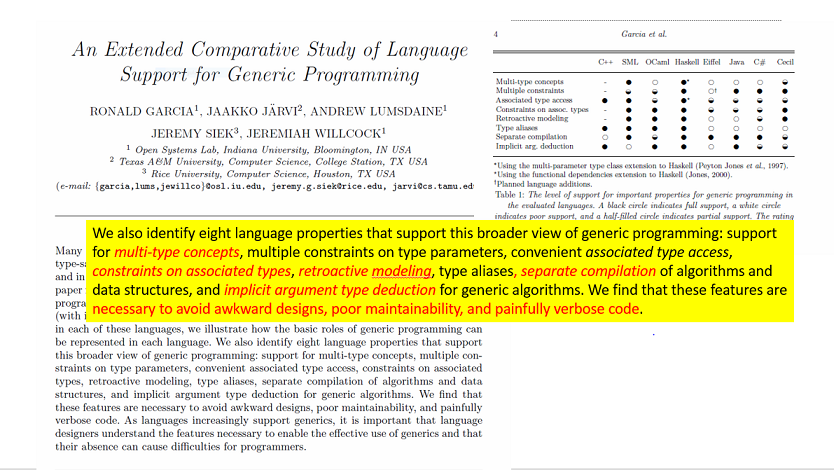
\includegraphics{./images/comparison.png}

--

\subsection{\texorpdfstring{\textbf{How
annoying!}}{How annoying!}}\label{how-annoying}

\begin{center}\rule{0.5\linewidth}{\linethickness}\end{center}

\subsection{Introduction}\label{introduction}

Type classes are an immensely popular and productive feature of Haskell.

(Almost as good as modules, sometimes better!)

So good, other languages have stolen them:

\begin{itemize}
\tightlist
\item
  \sout{C++ concepts} (for perf!)
\item
  Scala \emph{implicits}
\item
  Rust \emph{traits}
\item
  Swift \emph{protocols}
\item
  Coq (2 variants),Agda, Clean\ldots{}.
\end{itemize}

--

But not C\# or F\#.

--


\includegraphics{./images/wecandoit.png}

\begin{center}\rule{0.5\linewidth}{\linethickness}\end{center}

\subsection{This talk:}\label{this-talk}

We add type classes to C\# using a cheap coding trick that is

\begin{itemize}
\tightlist
\item
  type preserving (no yucky erasure)
\item
  efficient (thanks to .NET's run-time code specialiation)
\item
  essentially free (zero VM modifications required)
\item
  modular
\end{itemize}

The same technique works interoperably for F\# etc.

For C\#, we call a type class a \emph{concept} and an instance an
\emph{instance}.

(In F\#, a type class is called \emph{trait} and an instance
\emph{witness}).

\emph{Concept C\#}\\
and \emph{Trait F\#}\\
are implemented as open source prototypes.

\url{https://github.com/MattWindsor91/roslyn/blob/master/README.md}

\begin{center}\rule{0.5\linewidth}{\linethickness}\end{center}

\subsection{Recap: Haskell Type
Classes}\label{recap-haskell-type-classes}

Type classes are an abstraction mechanism for describing generic
algorithms.

A \emph{type class} is a predicate on types that specifies a set of
required operations by signature.

A \emph{class instance} declares class membership of a type by
implementing each operation.

Type classes form hierarchies with \emph{inheritance} and
\emph{subsumption}.

A \emph{generic instance} defines \emph{families} of instances,
predicated on class membership.

\begin{center}\rule{0.5\linewidth}{\linethickness}\end{center}

\subsection{Why should .NET care?}\label{why-should-.net-care}

Instance declarations are decoupled from their types (unlike an OO
class' interfaces).

Type classes can have less overhead than OO abstractions. Even zero
overhead.

Type classes allow efficient abstraction over numeric types (sorely
missing in .NET).

\begin{center}\rule{0.5\linewidth}{\linethickness}\end{center}

\subsection{\texorpdfstring{\sout{``Static Interface Methods for the
CLR''}}{Static Interface Methods for the CLR}}\label{static-interface-methods-for-the-clr}

.NET team previously proposed and prototyped ``Static Interface Methods
for the CLR'',\\
driven by customer demand for \emph{efficient} abstraction over numeric
types.

Why didn't this proposal make it?

\begin{itemize}
\tightlist
\item
  It required both runtime \& framework changes (too expensive).
\item
  It has soundness issues (too risky).
\end{itemize}

Our approach:

\begin{itemize}
\tightlist
\item
  requires \emph{no} changes to the runtime or frameworks.
\item
  Is \emph{sound by construction} (due to evidence passing).
\end{itemize}

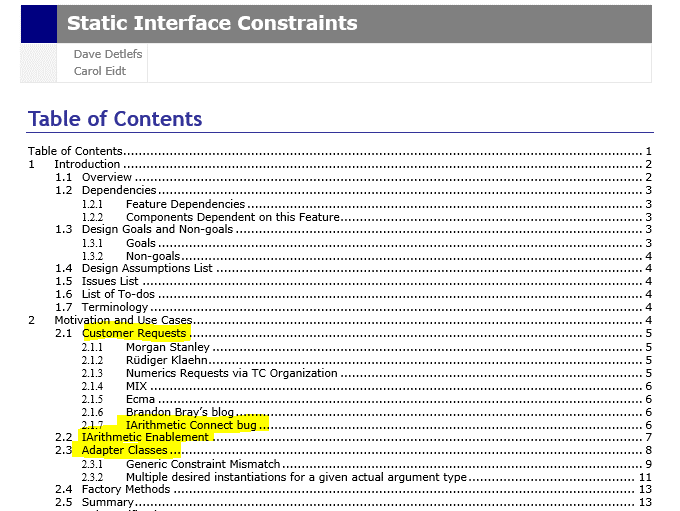
\includegraphics{./images/staticinterfaces.png}

\begin{center}\rule{0.5\linewidth}{\linethickness}\end{center}

\subsection{Generics Recap}\label{generics-recap}

define \emph{Generics}: object-oriented lingo for \emph{F-bounded
parametric polymorphism}

\begin{center}\rule{0.5\linewidth}{\linethickness}\end{center}

\subsection{Java/JVM Generics}\label{javajvm-generics}

Java generics are a fiction of the compiler's imagination.

Compiled by ``erasing type parameters to their bounds or
\lstinline!object!''.

\emph{Erasure Semantics} means the Java VM knows nothing about type
parameters, let alone their instantiations .

All instantiations of generic type must have the same least common
denominator representation (a heaper pointer).

Because of erasure, Java has to rule out certain (arguably useful!)
constructs:

\begin{lstlisting}[language=Java]
new T()         // illegal Java allocation
new T[100]      // illegal Java array construction
(T) o           // illegal Java cast 
(List<Int>) o   // illegal Java cast
List<Int>       // legal, but boxes every entry (fat and slow)
List<int>       // illegal, instantiation not pointer sized 
sizeof(List<Int>) == sizeof(List<Bool)) == sizeof(List<String>) 
\end{lstlisting}

\begin{center}\rule{0.5\linewidth}{\linethickness}\end{center}

\subsection{C\#/F\#/.NET Generics}\label{cf.net-generics}

In C\#, Generics are built into the vm (dedicated bytecodes \&\\
type metadata).

Compiled by ``passing types at runtime''.

\emph{Type Passing} means the virtual machine knows about type
parameters and their instantiations at runtime.

The runtime is free to choose different sized representations for
different types, even when used as type arguments.

\begin{lstlisting}
new T()         // legal C#
new T[100]      // legal C#
(T)o            // legal C#
(List<int>) o   // legal C#
List<byte>       // legal, note instantiation not pointer sized 
sizeof(List<int>) =/= sizeof(List<bool>) =/= sizeof(List<String>)
// even THIS is ok (though it arguably isn't...)
if (typeof<T> == typeof<int>) 
   Write("I just broke parametericity!");  
\end{lstlisting}

\begin{center}\rule{0.5\linewidth}{\linethickness}\end{center}

\subsection{Code Specialization}\label{code-specialization}

Importantly, for performance, the CLR generates specialised code for
particular instantiations (Kennedy \& Syme, 2001)

Types comes in two flavours:

\begin{itemize}
\tightlist
\item
  \emph{value types} (scalar primitives \& user defined structures).\\
  Cheaply stack-allocated, passed by value.
\item
  \emph{reference types} (objects \& arrays).\\
  Expensively heap-allocated, passed by reference.
\end{itemize}

Type parameters range over/can be instantiated with both flavours.

Code instantiated at \emph{reference} (ie. heap) types
(\lstinline!object!,\lstinline!string!, \lstinline!int[]!) is
\emph{shared} between all reference type instantiations (with some
indirection\\
for type specific operations) (to avoid code bloat).

Code instantiated at \emph{value} types (\lstinline!int16!,
\lstinline!int32!, \lstinline!point!) is \emph{specialized} for each
instantiation.

Code instantiated at mixtures of reference and non-reference types is
``partially'' specialized (it's complicated).

\begin{center}\rule{0.5\linewidth}{\linethickness}\end{center}

\subsection{Benefits of
Specialization}\label{benefits-of-specialization}

Specialization typically happens \emph{just-in-time} (i.e.~at run time,
at first unseen instantiation).

Specialization replaces statically unknown representation sizes by
dynamically known ones.

Like static inlining, type specialization can turn indirect calls (to
\emph{unknown} functions) into faster, direct calls to \emph{known}
functions.

Futhermore, \emph{known} functions can be \emph{inlined}, removing
function call overhead altogether and exposing yet more optimizations.

(An run time version of C++'s compile time type specialization.)

\begin{center}\rule{0.5\linewidth}{\linethickness}\end{center}


\includegraphics{./images/CheapTrick.png}

\begin{center}\rule{0.5\linewidth}{\linethickness}\end{center}

\subsection{Haskell Type Classes}\label{haskell-type-classes}

We represent a Haskell type class, e.g.

\begin{lstlisting}[language=Haskell]
  class Eq a where 
    (==) :: a -> a -> Bool
\end{lstlisting}

as a \emph{generic} C\# \emph{interface}:

\begin{lstlisting}
  interface Eq<A>
  {
    bool Equal(A a, A b);
  }
\end{lstlisting}

\emph{Concept C\#} just adds a distinctive \lstinline!concept! keyword.

\begin{lstlisting}
  concept Eq<A>
  {
    bool Equal(A a, A b);
  }
\end{lstlisting}

\begin{center}\rule{0.5\linewidth}{\linethickness}\end{center}

\subsection{Haskell Overloads}\label{haskell-overloads}

The Haskell declaration of class \lstinline!Eq a! implicitly declares
the overload:

\begin{lstlisting}[language=Haskell]
    (==) :: (Eq a) => a -> a -> Bool  -- note the added constraint!
\end{lstlisting}

In C\#, an overload can be encoded as a generic static method,
parameterized by an additional type parameter \lstinline!'EqA!.

C\#

\begin{lstlisting}
static class Overloads {
  public static bool Equal<A,EqA>(A a,A b) where EqA:struct,Eq<A> =>
    default(EqA).Equal(a, b);
}
\end{lstlisting}

The ordinary type parameter \lstinline!EqA! is:

\begin{itemize}
\tightlist
\item
  constrained to be a \lstinline!struct! (allocable on the stack);
\item
  bounded by its interface (\lstinline!EqA: Eq<A>!);
\item
  a named \emph{witness} for the constraint \lstinline!Eq<A>!.
\end{itemize}

(think \lstinline!Equal!:
\lstinline!forall A, EqA : Eq<A>. A -> A -> bool!)

\begin{quote}
\emph{Haskell dictionary value \textasciitilde{} C\# witness type}
\end{quote}

\begin{center}\rule{0.5\linewidth}{\linethickness}\end{center}

\subsection{Types as Dictionaries}\label{types-as-dictionaries}

Haskell's dictionary translation compiles == to a function with a
implicit \emph{dictionary} argument

\begin{lstlisting}[language=Haskell]
    (==) :: (Eq a) => a -> a -> Bool  -- note the added constraint!
    == (d::Eq A) (a::a) (b::a) = d.== a b  
    --  ^ d is an implicit dictionary parameter providing d.==
\end{lstlisting}

Look closely at the C\# encoding of Haskell's (==)

\begin{lstlisting}
  public static bool Equal<A,EqA>(A a,A b) where EqA:struct,Eq<A> =>
    default(EqA).Equal(a, b);
\end{lstlisting}

Where is the \emph{value} parameter for the ``dictionary'' \lstinline!d!
that Haskell would insert?

--

We don't need to pass dictionary values - just dictionary \emph{types}!

In C\#, primitive \lstinline!default(T)! has type \lstinline!T! and
returns a default value.

Using \lstinline!default(T)!, we can always create a dictionary value
from the corresponding dictionary type!

(The \lstinline!struct! constraint ensures dictionary value are
non-\lstinline!null!; no call can fail.)

\begin{center}\rule{0.5\linewidth}{\linethickness}\end{center}

\subsection{\ldots{} Types as
Dictionaries}\label{types-as-dictionaries-1}

Calling `default(T)' is gross (esp. when `T' is large)!

Instead of the C\#:

\begin{lstlisting}
public static bool Equal<A,EqA>(A a,A b) where EqA:struct,Eq<A> =>
  default(EqA).Equal(a, b);
\end{lstlisting}

Concept C\# allows methods with `implicit' type parameters introducing
static methods:

\begin{lstlisting}
public static bool Equal<A,implicit EqA>(A a,A b) where EqA:Eq<A> =>
  Equal(a, b); 
\end{lstlisting}

and instead of \lstinline!default(EqA).Equal(a, b)! we can just write
\lstinline!Equal(a,b)!.

The \lstinline!implicit! keyword declares a dictionary type parameter
whose:

\begin{itemize}
\tightlist
\item
  methods are available sans qualification;
\item
  instantiations are inferred from the user's concept/instance
  hierarchy.
\end{itemize}

(NB \lstinline!EqA.Equal(a, b)! is ok too).

\begin{center}\rule{0.5\linewidth}{\linethickness}\end{center}

\subsection{Haskell Instances}\label{haskell-instances}

A Haskell ground instance, eg.

\begin{lstlisting}[language=Haskell]
  instance Eq Integer where 
    x == y                =  x `integerEq` y
\end{lstlisting}

is translated to a C\# \emph{struct} implementing a concept
(i.e.~interface).

\begin{lstlisting}
  struct EqInt : Eq<int>  {
    public bool Equal(int a, int b)  => a == b; 
  }
\end{lstlisting}

The struct is empty (think \lstinline!unit!) but (!) has associated
code.

In Concept C\#, we use the instance keyword instead:

\begin{lstlisting}
  instance EqInt : Eq<int> {
    public bool Equal(int a, int b)  => a == b; 
  }
\end{lstlisting}

Altough they compile to struct declarations, instances are used
specially, to instantiate\\
\lstinline!implicit! type parameters.

\begin{center}\rule{0.5\linewidth}{\linethickness}\end{center}

\subsection{Generic Instances\ldots{}}\label{generic-instances}

Haskell's generic instances define \emph{families} of instances.

E.g.

Given an equality type \lstinline!a!, we can define an equality\\
on \emph{lists} of \lstinline!a! (written \lstinline![a]!):

\begin{lstlisting}[language=Haskell]
  instance (Eq a) => Eq [a] where 
       nil == nil      = true
    (a:as) == (b:bs)   = (a == b) && (as == bs)
         _ == _        = false
\end{lstlisting}

\begin{center}\rule{0.5\linewidth}{\linethickness}\end{center}

\subsection{\ldots{}Generic Instances}\label{generic-instances-1}

We can represent a Haskell \emph{parameterized instance} as a
\emph{generic struct},\\
implementing an interface but parameterized by constrained type
parameters.

Substituting, for simplicity, arrays for lists in CS we can write:

\begin{lstlisting}
struct EqArray<A, EqA> : Eq<A[]> where EqA : struct, Eq<A> {
  public bool Equal(A[] a, A[] b) {
    if (a.Length != b.Length) return false;
    for (int i = 0; i < a.Length; i++)
      if (!(default(EqA).Equal(a[i], b[i]))) return false;
    return true;
  }
}
\end{lstlisting}

Concept C\#:

\begin{lstlisting}
instance EqArray<A, implicit EqA> : Eq<A[]> where EqA : Eq<A> {
  bool Equal(A[] a, A[] b) {
    if (a.Length != b.Length) return false;
    for (int i = 0; i < a.Length; i++)
      if (!Equal(a[i], b[i])) return false;
    return true;
  }
}
\end{lstlisting}

\begin{center}\rule{0.5\linewidth}{\linethickness}\end{center}

\subsection{Constructing Evidence}\label{constructing-evidence}

Derived instances allow Haskell to automatically construct instances as
evidence for constraints:

\begin{lstlisting}[language=Haskell]
  --- Since Eq Integer and Eq a => Eq (List a),
  --- we have Eq (List Integer) hence Eq (List (List Integer))
   
   [[1],[2,2],[3,3,3]] == [[3,3,3],[2,2],[1]]  -- typechecks!
\end{lstlisting}

In C\#, \lstinline!EqInt:Eq<int>! so
\lstinline!EqArray<int,EqInt>:Eq<int[]>! so
\lstinline!EqArray<int[],EqArray<int,EqInt>>:Eq<int[][]>!.

In C\#, dictionary type arguments cannot be inferred\ldots{} they
usually don't occur elsewhere in the type!

\begin{lstlisting}
   bool Equal<A,EqA>(A a, A b) where EqA: struct, Eq<A>;

   Equal( {{1},{1,2},{1,2,3}}, {{1,2,3},{1,2},{1}} ) 
     // type error, C# can't infer type arguments!
   
   Equal<int[][], EqArray<int[],EqArray<int,EqInt>> >
    ( {{1},{1,2},{1,2,3}}, {{1,2,3},{1,2},{1}} ) 
     // typechecks (but kills the programmer)
\end{lstlisting}

Programming in the encoding requires an intolerable amount of explicit
type instantiation.

\begin{center}\rule{0.5\linewidth}{\linethickness}\end{center}

\subsection{Instance Inference}\label{instance-inference}

No programmer should write this crap!

In Concept C\#, we extend type argument inference so:

\begin{itemize}
\tightlist
\item
  ordinary and implicit type arguments can be omitted and inferred;
\item
  ordinary type arguments can be provided but implicit type arguments
  can be omitted and inferred;
\item
  ordinary and implicit type arguments can be provided (when necessary).
\end{itemize}

Concept C\#:

\begin{lstlisting}
  bool Equal<A,implicit EqA>(A a, A b) where EqA:Eq<A>;

  Equal({{1},{1,2},{1,2,3}},{{1,2,3},{1,2},{1}}) 
   // type checks: implicit parameter inferrable from argument type

  Equal< int[][] >({{1},{1,2},{1,2,3}},{{1,2,3},{1,2},{1}}) 
   // also checks(used when C# type inference fails)

  Equal< int[][], EqArray<int[],EqArray<int,EqInt>> >
       ({{1},{1,2},{1,2,3}},{{1,2,3},{1,2},{1}})
   // also checks (used when implicit inference fails).
\end{lstlisting}

\subsection{\texorpdfstring{`implicit' type parameters are inferred
using instance driven backchaining, similar to
Haskell.}{implicit type parameters are inferred using instance driven backchaining, similar to Haskell.}}\label{implicit-type-parameters-are-inferred-using-instance-driven-backchaining-similar-to-haskell.}

\subsection{Derived Operations}\label{derived-operations}

We translate Haskell's qualified types as extra, bounded type parameters
denoting witness parameters.

For example, equality based list membership in Haskell is defined as
follows:

\begin{lstlisting}[language=Haskell]
  elem :: Eq a => a -> [a] -> bool
  elem x []      = False
  elem x (y:ys)  = x==y || (elem x ys)  
\end{lstlisting}

In C\#, we can define:

\begin{lstlisting}
static bool Elem<A,EqA>(A x, A[] ys) where EqA : struct, Eq<A> {
  for (int i = 0; i < ys.Length; i++)  
    if default(EqA).Equal(x, ys[i])) return true;
  return false;
}
\end{lstlisting}

Concept C\#:

\begin{lstlisting}
static bool Elem<A,implicit EqA>(A x, A[] ys) where EqA : Eq<A> {
  for (int i = 0; i < ys.Length; i++) 
    if (Equal(x, ys[i])) return true;
  return false;
}
\end{lstlisting}

\begin{center}\rule{0.5\linewidth}{\linethickness}\end{center}

\subsection{Example: Numeric types}\label{example-numeric-types}

Haskell has a rich numeric hierarchy (think \lstinline!IArithmetic!)

\begin{lstlisting}[language=Haskell]
  class Num a where
    Add: a -> a -> a
    Mult: a -> a -> a
    Neg: a -> a
  
  instance Num Integer where
    Add a b = a + b
    Mult a b = a * b
    Neg a  = -a
  
  instance Num Float where 
    ...
\end{lstlisting}

\begin{center}\rule{0.5\linewidth}{\linethickness}\end{center}

\subsection{\ldots{} Example: Numeric
types}\label{example-numeric-types-1}

C\#:

\begin{lstlisting}
interface Num<A> {
    A Add(A a, A b);
    A Mult(A a, A b);
    A Neg(A a);
  }
struct NumInt : Num<int> {
    public int Add(int a, int b) => a + b; 
    public int Mult(int a, int b) => a * b; 
    public int Neg(int a) => -a;
}
\end{lstlisting}

Concept C\#:

\begin{lstlisting}
concept Num<A> {
    A Add(A a, A b);
    A Mult(A a, A b);
    A Neg(A a);
}
instance NumInt : Num<int> {
    int Add(int a, int b) => a + b; 
    int Mult(int a, int b) => a * b; 
    int Neg(int a) => -a;
 }      
\end{lstlisting}

\begin{center}\rule{0.5\linewidth}{\linethickness}\end{center}

\subsection{Type Class Inheritance}\label{type-class-inheritance}

Haskell supports (multiple) inheritance of super classes.

\begin{lstlisting}[language=Haskell]
  class (Eq a) => Num a where
    Add: a -> a -> a
    Mult: a -> a -> a
    Neg: a -> a
\end{lstlisting}

\begin{itemize}
\tightlist
\item
  Forall types \lstinline!a!, \lstinline!Num a! derives from
  \lstinline!Eq a!.
\end{itemize}

(Is it just me or is Haskell's \lstinline!=>! the wrong-way round?).

In C\#, we instead use (multiple) interface inheritance C\#:

\begin{lstlisting}
interface Num<A> : Eq<A> {
  A Add(A a, A b);
  A Mult(A a, A b);
  A Neg(A a);
}
struct NumInt : Num<int> {
  public bool Equal(int a, int b) => default(EqInt).Equal(a, b);
  public int Add(int a, int b) => a + b;
  public int Mult(int a, int b) => a * b; 
  public int Neg(int a) => -a;
}
\end{lstlisting}

\begin{center}\rule{0.5\linewidth}{\linethickness}\end{center}

\subsection{\ldots{} Inheritance}\label{inheritance}

Concept C\#:

\begin{lstlisting}
concept Num<A> : Eq<A> {
  A Add(A a, A b);
  A Mult(A a, A b);
  A Neg(A a);
}
instance NumInt : Num<int> {
  bool Equal(int a, int b) => EqInt.Equal(a, b); 
       // named instance EqInt useful here (c.f. Haskell)
  int Add(int a, int b) => a + b;
  int Mult(int a, int b) => a * b; 
  int Neg(int a) => -a;
}
\end{lstlisting}

\begin{itemize}
\tightlist
\item
  Haskell class inheritance \textasciitilde{} C\# interface inheritance
\end{itemize}

\begin{center}\rule{0.5\linewidth}{\linethickness}\end{center}

\subsection{Subsumption \ldots{}}\label{subsumption}

Subsumption derives (evidence for) a class from (evidence for) its
subclasses.

\begin{lstlisting}[language=Haskell]
    equal :: (Eq a) => a -> a -> Bool

    square :: (Num a) => a -> a 
    square a = a * a

    memsq :: (Num a) => [a] -> a -> Bool
    memsq nil a = false
    memsq (h:t) a =     equal h (square a) 
                     -- ^^^^ legal coz Num a |= Eq a 
                     || memsq h t
\end{lstlisting}

\begin{center}\rule{0.5\linewidth}{\linethickness}\end{center}

\subsection{\ldots{} Subsumption}\label{subsumption-1}

C\#:

\begin{lstlisting}
static bool Equal<EqA, A>(A a, A b) where EqA : struct, Eq<A> 
  => default(EqA).Equal(a, b);
static A Square<A,NumA>(A a) where NumA : struct, Num<A> 
  => default(NumA).Mult(a, a);
static bool MemSq<A,NumA>(A[] a_s, A a) where NumA: struct, Num<A>
{ for (int i = 0; i < a_s.Length; i++) 
    if (Equal<A,NumA>(a_s[i], Square<NumA, A>(a))) return true;
             /*  ^^^^ legal only because NumA : Num<A> : Eq<A> */
  return false;
}
\end{lstlisting}

Concept C\#:

\begin{lstlisting}
static bool Equal<A,implicit EqA>(A a, A b) where EqA : Eq<A> 
  => Equal(a, b);
static A Square<A,implicit NumA>(A a) where NumA: Num<A> 
  => Mult(a, a);
static bool MemSq<A,implicit NumA>(A[] a_s, A a) where NumA: Num<A>
{ for (int i = 0; i < a_s.Length; i++) 
    if (Equal(a_s[i], Square(a))) return true;
     /*  ^^^^ legal only because  NumA : Num<A> : Eq<A> */
  return false;
}
\end{lstlisting}

\begin{center}\rule{0.5\linewidth}{\linethickness}\end{center}

\subsection{The logical perspective}\label{the-logical-perspective}

\begin{itemize}
\tightlist
\item
  concepts define \emph{predicates}
\item
  instances define \emph{axioms} \& \emph{inference rules}
\item
  well-formed types are \emph{proofs} of predicates
\item
  proof defines semantics
\item
  (choice of proof \textasciitilde{}\textasciitilde{} choice of
  semantics)
\end{itemize}

\begin{lstlisting}
concept Eq<A>                          Eq: Type -> Prop

instance EqInt : Eq<int>               ------- (EqInt)
                                       Eq<int>
  
instance EqArray<A,implicit EqA>       EqA:Eq<A>
         where EqA:Eq<A>               --------- (EqArray<A,EqA>)
         : Eq<A>                       Eq<A[]>
\end{lstlisting}

Haskell imposes restrictions that ensures proofs are unique and provide
unambiguous \sout{code} semantics.

Concept C\# could do this too \emph{or} be more flexible:

\begin{itemize}
\tightlist
\item
  insist on unambiguous inferences
\item
  but allow explicit disambiguation by instantiation (when inference
  fails)
\end{itemize}

\begin{center}\rule{0.5\linewidth}{\linethickness}\end{center}

\section{Perf}\label{perf}

\begin{center}\rule{0.5\linewidth}{\linethickness}\end{center}

\subsection{MSIL ByteCode}\label{msil-bytecode}

\begin{lstlisting}
public static bool Equal<A,EqA>(A a,A b) where EqA:struct,Eq<A> =>
  default(EqA).Equal(a, b);
\end{lstlisting}

Compiles to (something like) CIL generic bytecode:

\begin{lstlisting}[language=C]
.method public static bool Equal<A, 
                                 struct .ctor(class Eq<!!A>) EqA> 
   (!!A a,!!A b) 
   cil managed {
   .locals init ([0] !!EqA loc1)
   ldloca.s loc1      // stack allocate dictionary
   initobj !!EqA      // initialize (empty) dictionary
   ldloca.s loc1      // load address of dictionary onto stack
   ldarg.0            // load argument 1   
   ldarg.1            // load argument 2
   constrained. !!EqA // pseudo virtual call through dictionary
   callvirt instance bool class Eq<!!A>::Equal(!0, !0) 
   ret
}
\end{lstlisting}

The \lstinline!callvirt! instruction is typically used for an indirect
call to a virtual method.

When actual type \lstinline!EqA! is a struct, due to specialization, the
callee is always known and often inlined.

\begin{center}\rule{0.5\linewidth}{\linethickness}\end{center}

\subsection{Performance}\label{performance}

Evaluating a polynomial \lstinline!f(x:T) = x*x + x + (T)666! (in C\#),

where \lstinline!T!=\lstinline!int!, \lstinline!double!,
\lstinline!Class3D!, \lstinline!Struct3D!.

(We evaluate \lstinline!f(x)! at \lstinline!1m! values of \lstinline!x!
using the BenchmarkDotNet harness.)

\begin{center}\rule{0.5\linewidth}{\linethickness}\end{center}

\begin{lstlisting}
T ConceptGenericOpt<T, NumT>() where NumT : struct, Num<T> {
  NumT NI = default(NumT);
  T y = NI.FromInteger(0);
  T c = NI.FromInteger(666);
  for (int i = 0; i < n; i++) {
    T x = NI.FromInteger(i);
    y = NI.Plus(NI.Plus(NI.Mult(x,x),x), c);
  }
  return y;
}
\end{lstlisting}

Competing implementations:

\begin{itemize}
\tightlist
\item
  Baseline: non generic, hand-specialized code (one per T)
\item
  AbstractClass: generic class based (OOP style)
\item
  Interface: generic interface based (OOP style)
\item
  Delegate: generic, first-class function based (OOP/FP style)
\item
  Instance: concept based (one dictionary value per call)
\item
  OptimizedInstance: optimized concept based (CSE on dictionaries)
  (shown above)
\item
  OptimizedInstanceInlined: optimized concept based (CSE on
  dictionaries) with C\# static operator definitions inlined in witness
  declaration.
\end{itemize}

\begin{center}\rule{0.5\linewidth}{\linethickness}\end{center}

\subsection{Relative Performance at Scalar
types}\label{relative-performance-at-scalar-types}

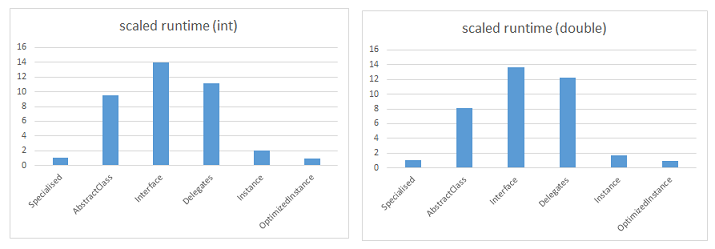
\includegraphics{./images/perf1.png}

(lower is better - ideally leftmost baseline (non-generic,
hand-specialized code) equals rightmost generic concept code.

At scalar primitive value type instantiations, concept performance is:

\begin{itemize}
\tightlist
\item
  as good as hand specialised code,
\item
  at least \emph{8-14x faster} than standard OO abstractions.
\end{itemize}

\begin{center}\rule{0.5\linewidth}{\linethickness}\end{center}

\subsection{Relative Performance at Compound
Types}\label{relative-performance-at-compound-types}

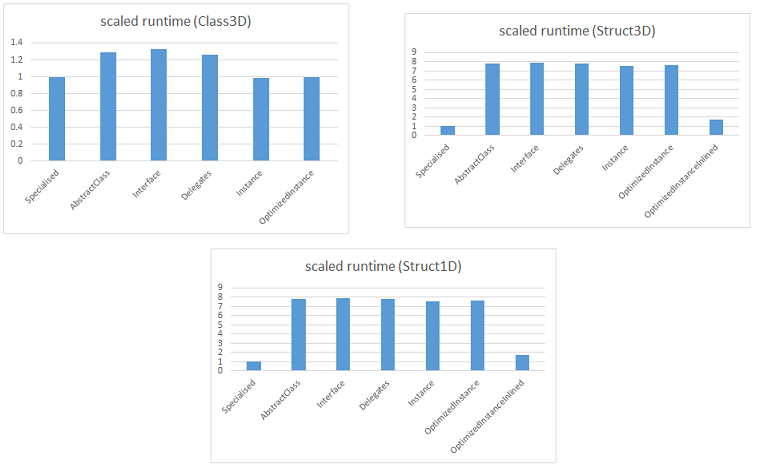
\includegraphics{./images/perf2.png}

(lower is better - ideally leftmost baseline equals rightmost generic,
concept code.

At 3-field class and struct instantiations, performance can be competive
with hand specialised code,\\
1.4-8x faster than OO abstractions (if we are careful to inline).

\begin{center}\rule{0.5\linewidth}{\linethickness}\end{center}

\subsection{x86 (DEBUG)}\label{x86-debug}

This, in outline, is the x86 code jitted at
\lstinline!NumInt:Num<int>!:\\
The real code is \emph{64 lines} of suboptimal masm (yuck).

\begin{lstlisting}
    696:             NumT NI = default(NumT);
    01140628  lea         eax,[ebp-10h]  
    0114062B  mov         byte ptr [eax],0  
    697:             T y = NI.FromInteger(0);
... 01140633  call        dword ptr ds:[0C65E78h]   ...
    698:             T c = NI.FromInteger(666);
... 0114064A  call        dword ptr ds:[0C65E78h]   ...  
    699:             for (int i = 0; i < n; i++) {
    700:                 T x = NI.FromInteger(i);
... 01140668  call        dword ptr ds:[0C65E78h]  ...
    701:                 y = NI.Plus(NI.Plus(NI.Mult(x,x),x), c);
... 0114068C  call        dword ptr ds:[0C65E8Ch]  ... 
... 0114069E  call        dword ptr ds:[0C65EA0h]  ...  
... 011406B0  call        dword ptr ds:[0C65EA0h]  ...
    702:             }
    703:             return y;
    704:         }
    011406E4  mov         eax,dword ptr [ebp-28h]  ... 
... 011406ED  ret  
\end{lstlisting}

Notice this still has 4 \emph{call} instructions in the inner loop - the
cost of abstraction!

But this is debug code, the \emph{optimizing} JIT does \emph{much}
better \ldots{}

\begin{center}\rule{0.5\linewidth}{\linethickness}\end{center}

\subsection{x86 (RELEASE)}\label{x86-release}

This is the optimised code jitted at \lstinline!NumInt:Num<int>!.

\begin{lstlisting}
   696:             NumT NI = default(NumT);
00007FFD8BF85110  sub         rsp,8  
00007FFD8BF85114  xor         eax,eax  
00007FFD8BF85116  mov         qword ptr [rsp],rax  
00007FFD8BF8511A  mov         byte ptr [rsp],0  
00007FFD8BF8511E  xor         eax,eax  
   699:             for (int i = 0; i < n; i++) {
00007FFD8BF85120  xor         edx,edx  
00007FFD8BF85122  mov         ecx,dword ptr [7FFD8BFC3B38h]  
00007FFD8BF85128  test        ecx,ecx  
00007FFD8BF8512A  jle         00007FFD8BF8513E  
00007FFD8BF8512C  mov         eax,edx  
00007FFD8BF8512E  imul        eax,edx  
00007FFD8BF85131  add         eax,edx  
00007FFD8BF85133  add         eax,29Ah  
00007FFD8BF85138  inc         edx  
00007FFD8BF8513A  cmp         edx,ecx  
00007FFD8BF8513C  jl          00007FFD8BF8512C  
00007FFD8BF8513E  add         rsp,8  
00007FFD8BF85142  ret  
\end{lstlisting}

\begin{itemize}
\tightlist
\item
  Notice this is straight-up arithmetic code! Just 18 lines of masm (was
  64 lines)
\item
  \emph{No} function calls/stack manipulation remain! \emph{Way faster}
  than debug code.
\item
  Dictionary initialization remains but the dictionary is dead and could
  be deleted)
\item
  Otherwise, code quality as good as hand-specialized code.
\end{itemize}

\begin{center}\rule{0.5\linewidth}{\linethickness}\end{center}

\subsection{Sugar: Operator
Overloading}\label{sugar-operator-overloading}

Even if efficient, few will write generic arithmetic code if they can't
use numeric syntax, i.e.~operators.

\begin{lstlisting}
public A F<A,implicit NumA>(x) where NumA:Num<A> =>            
   Plus( Plus( Mult(x,x), x),FromInteger(666)); // x*x + x + 666
\end{lstlisting}

Concept C\# supports natural operator declarations and definitions:

\begin{lstlisting}
concept Num<A> {
        A operator +(A a, A b);
        A operator *(A a, A b);
        A operator -(A a);
        implicit operator A(int i); //NYI
}
instance NumInt : Num<int> {
        int operator +(int a, int b) => a + b;
        int operator *(int a, int b) => a * b;
        int operator -(int a) => -a;
        implicit operator int(int i) => i;
}
public A F<A,implicit NumA>(x) where NumA:Num<A> =>         
     x*x + x + 666; // much nicer!
\end{lstlisting}

\begin{center}\rule{0.5\linewidth}{\linethickness}\end{center}

\subsection{Syntactic Design Space}\label{syntactic-design-space}

Option 1: Haskell-like - anonymous instances, anonymous dictionary
parameters (never implemented)

\begin{lstlisting}
instance Eq<int> {
    int Equal(int a, int b) => a == b;
}
static bool Equals<A>(A a, A b) where Eq<A> => a == b;
\end{lstlisting}

Concise, but \ldots{}

\begin{itemize}
\tightlist
\item
  anonymous instances prevent explicit instantiation
\item
  MSIL needs a name for the instance, so do other languages
\item
  bad for interop
\end{itemize}

\begin{center}\rule{0.5\linewidth}{\linethickness}\end{center}

\subsection{.. Syntactic Design
Space\ldots{}}\label{syntactic-design-space-1}

Option 2: Named instances with undeclared dictionary parameters

\begin{lstlisting}
instance EqInt : Eq<int> {
    int Equal(int a, int b) => a == b;
}
static bool Equal<A>(A a, A b) where EqA:Eq<A> => a == b;
\end{lstlisting}

\begin{itemize}
\tightlist
\item
  \lstinline!EqA! only occurs in constraint, not type parameters
\item
  what if we need to instantiate \lstinline!EqA! at call sites? What is
  \lstinline!Equal!'s true method signature?
\item
  better for interop
\end{itemize}

\begin{center}\rule{0.5\linewidth}{\linethickness}\end{center}

\subsection{.. Syntactic Design Space}\label{syntactic-design-space-2}

Option 3: Named instances, declared dictionary type parameters, marked
\lstinline!implicit!

\begin{lstlisting}
instance EqInt : Eq<int> {
    int Equal(int a, int b) => a == b;
}
static bool Equals<A,implicit EqA>(A a, A b) where EqA:Eq<A> =>
    a == b;
\end{lstlisting}

\begin{itemize}
\tightlist
\item
  unambiguous method signatures
\item
  best for interop
\end{itemize}

\begin{center}\rule{0.5\linewidth}{\linethickness}\end{center}

\subsection{Proposed Case Studies (In
Progress)}\label{proposed-case-studies-in-progress}

\begin{itemize}
\tightlist
\item
  Micro-benchmarks for perf (sorting \& arithmetic)
\item
  Automatic Differentiation in C\#/F\#, overloading arithmetic to
  compute function derivatives {[}1{]}
\item
  C\#, F\# renditions of Haskell Prelude, including numeric tower
\item
  C\# Generic QuickHull (one convex hull algorithm for generic vector
  spaces)
\end{itemize}

Future:

\begin{itemize}
\tightlist
\item
  C\# Generic Graph Library - Haskell used to trump C\#, does it still?
\item
  Pickling
\item
  Normalization by Evaluation
\item
  \ldots{} any suggestions?
\end{itemize}

{[}1{]}{[}``Conal Elliot, Beautiful Differentiation''{]}

\begin{center}\rule{0.5\linewidth}{\linethickness}\end{center}

\subsection{Summary}\label{summary}

\begin{center}\rule{0.5\linewidth}{\linethickness}\end{center}

\begin{longtable}[]{@{}lll@{}}
\toprule
\begin{minipage}[b]{0.14\columnwidth}\raggedright\strut
Haskell\strut
\end{minipage} & \begin{minipage}[b]{0.11\columnwidth}\raggedright\strut
C\#\strut
\end{minipage} & \begin{minipage}[b]{0.11\columnwidth}\raggedright\strut
Concept C\#\strut
\end{minipage}\tabularnewline
\midrule
\endhead
\begin{minipage}[t]{0.14\columnwidth}\raggedright\strut
type class\strut
\end{minipage} & \begin{minipage}[t]{0.11\columnwidth}\raggedright\strut
generic interface\strut
\end{minipage} & \begin{minipage}[t]{0.11\columnwidth}\raggedright\strut
generic concept\strut
\end{minipage}\tabularnewline
\begin{minipage}[t]{0.14\columnwidth}\raggedright\strut
instance\strut
\end{minipage} & \begin{minipage}[t]{0.11\columnwidth}\raggedright\strut
struct\strut
\end{minipage} & \begin{minipage}[t]{0.11\columnwidth}\raggedright\strut
instance\strut
\end{minipage}\tabularnewline
\begin{minipage}[t]{0.14\columnwidth}\raggedright\strut
derived instance\strut
\end{minipage} & \begin{minipage}[t]{0.11\columnwidth}\raggedright\strut
generic struct\strut
\end{minipage} & \begin{minipage}[t]{0.11\columnwidth}\raggedright\strut
generic instance\strut
\end{minipage}\tabularnewline
\begin{minipage}[t]{0.14\columnwidth}\raggedright\strut
type class inheritance\strut
\end{minipage} & \begin{minipage}[t]{0.11\columnwidth}\raggedright\strut
interface inheritance\strut
\end{minipage} & \begin{minipage}[t]{0.11\columnwidth}\raggedright\strut
concept inheritance\strut
\end{minipage}\tabularnewline
\begin{minipage}[t]{0.14\columnwidth}\raggedright\strut
overloaded operation\strut
\end{minipage} & \begin{minipage}[t]{0.11\columnwidth}\raggedright\strut
constrained generic method\strut
\end{minipage} & \begin{minipage}[t]{0.11\columnwidth}\raggedright\strut
generic method with implicit type parameters\strut
\end{minipage}\tabularnewline
\begin{minipage}[t]{0.14\columnwidth}\raggedright\strut
implicit dictionary construction\strut
\end{minipage} & \begin{minipage}[t]{0.11\columnwidth}\raggedright\strut
explicit type construction\strut
\end{minipage} & \begin{minipage}[t]{0.11\columnwidth}\raggedright\strut
implicit instance construction with explicit fallback\strut
\end{minipage}\tabularnewline
\begin{minipage}[t]{0.14\columnwidth}\raggedright\strut
implicit dictionary passing\strut
\end{minipage} & \begin{minipage}[t]{0.11\columnwidth}\raggedright\strut
explicit type passing\strut
\end{minipage} & \begin{minipage}[t]{0.11\columnwidth}\raggedright\strut
implicit type passing with explicit fallback\strut
\end{minipage}\tabularnewline
\begin{minipage}[t]{0.14\columnwidth}\raggedright\strut
constraint inference \& propagation\strut
\end{minipage} & \begin{minipage}[t]{0.11\columnwidth}\raggedright\strut
NA\strut
\end{minipage} & \begin{minipage}[t]{0.11\columnwidth}\raggedright\strut
NA\strut
\end{minipage}\tabularnewline
\bottomrule
\end{longtable}

\begin{center}\rule{0.5\linewidth}{\linethickness}\end{center}

\begin{center}\rule{0.5\linewidth}{\linethickness}\end{center}

\subsection{Take Home}\label{take-home}

\begin{itemize}
\tightlist
\item
  Haskell 98's type classes have a type preserving .NET representation.
\item
  Dictionaries can be manually constructed and provided or, better,
  inferred.
\item
  Generated code is efficient:

  \begin{itemize}
  \tightlist
  \item
    Dictionaries are empty (stack-allocated) structs.
  \item
    Dictionary allocation has zero runtime cost.
  \item
    CLR's code specialization ensures all dictionary calls are direct
    calls at runtime. Many are in-lined.
  \end{itemize}
\end{itemize}

\begin{center}\rule{0.5\linewidth}{\linethickness}\end{center}

\subsection{Future work:}\label{future-work}

\begin{itemize}
\tightlist
\item
  Exploit variance in interfaces (no Haskell analog).
\item
  Associated Types/Poor Man's Modules
\item
  JIT/Compiler comptimizations (sharing dictionary values, hoisting
  stack initialization out of loops).
\item
  Tech transfer (hearts and minds)
\item
  Justified, pluggable Types
\end{itemize}

\begin{center}\rule{0.5\linewidth}{\linethickness}\end{center}

\subsection{Links \& References}\label{links-references}

Concept C\#

\begin{itemize}
\tightlist
\item
  This document
  \url{https://github.com/MattWindsor91/roslyn/blob/master/concepts/docs/csconcepts.md}
\item
  C\# fork \url{https://github.com/MattWindsor91/roslyn}
\item
  Roslyn \url{https://github.com/dotnet/roslyn}.
\end{itemize}

Trait F\#

\begin{itemize}
\tightlist
\item
  F\# version
  \url{https://github.com/MattWindsor91/visualfsharp/blob/hackathon-vs/examples/fsconcepts.md}
\item
  F\# fork
  \url{https://github.com/MattWindsor91/visualfsharp/tree/hackathon-vs}
\end{itemize}

Papers (tiny subset)

\begin{itemize}
\tightlist
\item
  D. Gregor, J. Jarvi, J. Siek, B. Stroustrup, G. Dos Reis, and A.
  Lumsdaine. \emph{Concepts: Linguistic support for generic programming
  in C++}, OOPSLA'06.\\
  A. Kennedy and D. Syme. Design and implementation of generics for the
  .net common language\\
  runtime, PLDI 2001.
\item
  B. C. Oliveira, A. Moors, and M. Odersky. \emph{Type classes as
  objects and implicits}, OOPSLA '10.
\item
  S . Peyton Jones. \emph{Haskell 98 language and libraries : the
  revised report}. Cambridge University Press, May 2003.\\
  P. Wadler and S. Blott. \emph{How to make ad-hoc polymorphism less ad
  hoc}. POPL '89
\item
  D. Yu, A. Kennedy, and D. Syme. \emph{Formalization of generics for
  the .Net Common language Runtime.}, POPL 2004.
\end{itemize}


\section*{References}

\bibliographystyle{elsarticle-num}

\bibliography{sigproc} 
\end{document}
